\documentclass[12pt,a4paper]{report}
\synctex=1
\usepackage[utf8]{inputenc}
\usepackage[margin=2cm, top=1.5cm, bottom=2cm]{geometry}
\usepackage{graphicx}
\usepackage{libertine}
\usepackage{amsmath}
\usepackage{amssymb}
\usepackage{listings}
\usepackage{pgfornament}
\usepackage{eso-pic}
\usepackage{textcomp}
\usepackage{courier}
\usepackage[hangul]{kotex}

\title{
	\centering
	\pgfornament[width=12cm,color=teal]{84}\\
	\vspace{1cm}
	\fontsize{40}{40} \selectfont {소규모 사업자를 위한\\범용 예약 시스템 매뉴얼}
		\pgfornament[width=12cm,color=teal]{88}\\
	\vfill}
\author{
	\LARGE
	\begin{tabular}{rl}
		\hline
		교과목명 : & 자료구조와 실습\\
		담당교수 : & 정 준호 교수님\\
		학과 : & 불교학부 \\
		학번 : & 2016110056\\ 
		이름 : & 박승원\\
		날짜 : & \today\\
		\hline
	\end{tabular}\vspace{2cm}
	\\

\includegraphics[width=0.5\textwidth]{/home/zezeon/Dropbox/Photos/logo.jpg}
	}
\date{}


\linespread{1.3}

\begin{document}
\maketitle

%\includegrap

\newpage
\tableofcontents

\noindent
\chapter{인스톨}
\section{컴파일}
본 예약 시스템은 서버와 클라이언트 프로그램, 그래픽 프론트 엔드와 대화형 콘솔 프론트 엔드로 구성되어 있다.
이를 구현한 소스는 makefile 프로젝트이다.
이 중 그래픽 프론트 엔드는 Gtkmm라이브러리에 의존하며, 리눅스 환경과 윈도우즈 환경에서  Gtkmm 개발자용 버전이 인스톨된 경우 컴파일될 수 있다.
이를 제외한 나머지는 C, C++언어로 작성되었으며, 모든 표준 환경에서 컴파일 될 수 있다.
\section{파일 인스톨}
소스를 컴파일하면 네 개의 파일이 얻어진다. server, client, frontend, console\_frontend이다. server파일은 서버 컴퓨터에 복사하여 실행시키면 되고, 그 이외는 모두 클라이언트 컴퓨터에 복사하여 실행하면 된다. 서버와 클라이언트 컴퓨터는 같은 컴퓨터일 수도 있다.
\section{사용자 설정 파일}
클라이언트 컴퓨터에는 serverip.cfg라는 서버의 ip주소를 적어둔
\footnote{예를 들자면 서버와 클라이언트가 같은 경우는 127.0.0.1} 
한 줄 짜리 파일을 만들어 두어야 한다. 
이 주소로 클라이언트는 서버컴퓨터를 찾는다. 

서버와 클라이언트는 facility.txt라는 동일한 시설 설정 파일을 가져야 한다.
첫 줄부터 차례로 시설명이 한 줄에 하나씩 들어가야 한다.

이 설정 파일들은 모두 텍스트 파일이며, 실행 파일과 동일한 디렉토리에 있어야 한다.
\section{실행}
server는 백그라운드로 실행하는 것이 좋다. 클라이언트가 접속하기 위해 항상 실행된 상태이어야 한다.
client는 개별 프로그램으로 사용가능하기도 하지만, 프론트엔드가 주로 사용한다.
콘솔 대화형 프론트엔드는 커맨드라인에서 실행하면 된다.
그래픽 프론트엔드는 커맨드라인에서 스케일을 인자로 실행한다. ./frontend.x 100 이렇게 실행하면 한 시간을 대략 2cm 정도의 테이블 셀로 표현하며 인자가 없을 경우도 100을 인자로 준 것과 같이 동작한다. 

./frontend 100 실행 예

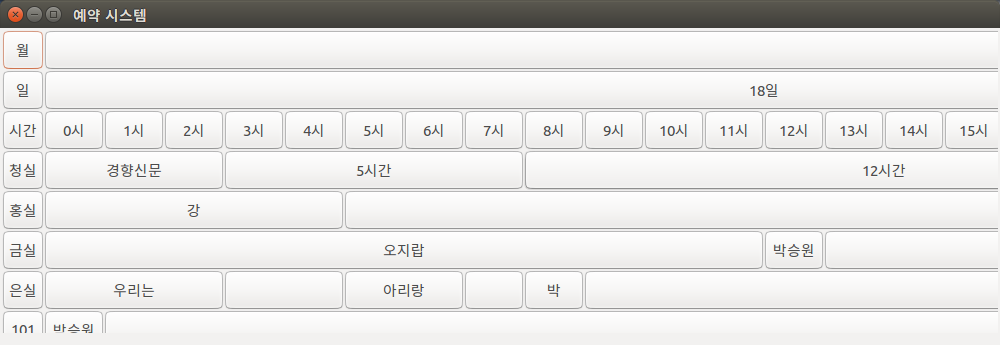
\includegraphics[width=0.9\textwidth]{exec.png}

200을 인자로 준 경우는 이 테이블 셀의 길이를 2배로 하고, 10을 인자로 준 경우는 1/10로 한다. 100보다 작은 인자를 주면 시간 표시가 사라지고 날짜 표시만 나온다. 5보다 작은 인자를 주면 날짜 표시도 사라지고 월 표시만 나온다.

./frontend 5 실행 예

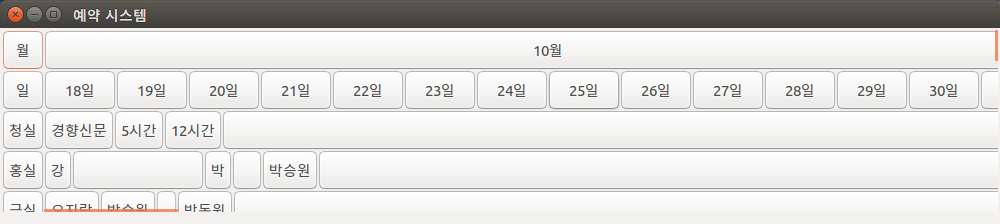
\includegraphics[width=0.9\textwidth]{mon.png}

위의 경우는 시간당 예약이 있는 시설에서 너무 작게 스케일하여 예약 시간이 밀린다.
그러므로, 자신의 업체에 맞는 스케일로 시간단위 예약을 하는 업체는 100 이상의 인자로 실행해야 한다. 배치 파일로 만들어 둘 수도 있다.
일 단위 예약일 경우는 위와 같이 5, 10 정도가 좋고,
월 단위 예약일 경우는 1 정도를 인자로 한다.

\chapter{사용법}

\section{그래픽 프론트 엔드}
그래픽 프론트 엔드는 매우 직관적으로 사용할 수 있다.
우선 상단에 시간이 월,일,시로 표시가 되며, 좌측에는 시설명이 표시된다.
시간과 시설이 만나는 지점에 있는 셀 들은 예약자의 이름을 시간에 맞게 표시한다.

좌우로 스크롤하면 다른 시간대를 볼 수 있고, 위 아래로 스크롤하면 다른 시설을 볼 수 있다.

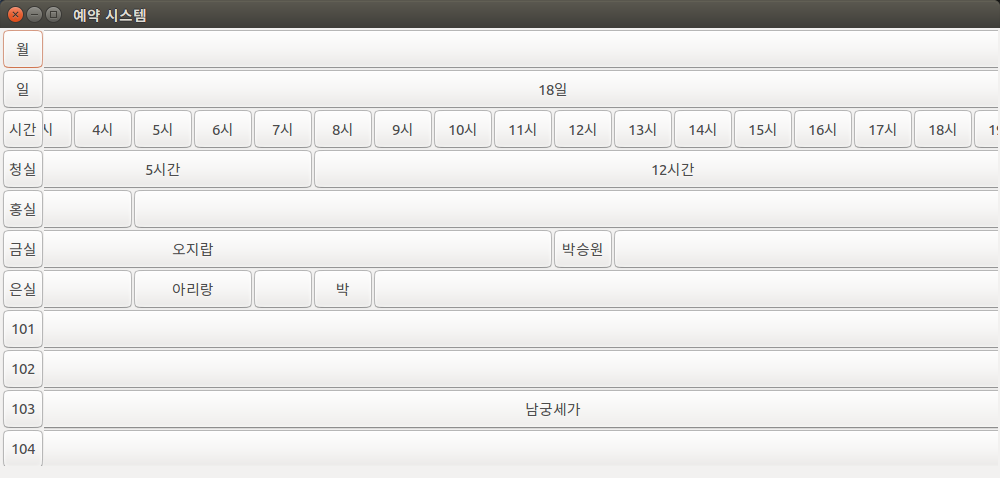
\includegraphics[width=\textwidth]{scroll.png}

예약자의 이름이 있는 칸을 클릭하면 연락처를 보여줌과 동시에 예약 취소가 가능하다.

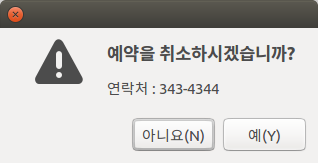
\includegraphics[width=0.3\textwidth]{cancel.png}

빈 칸을 클릭하면 그 칸에 맞는 시간을 초기화하여 예약을 입력할 수 있는 창이 뜬다.

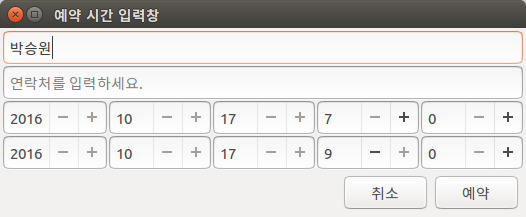
\includegraphics[width=0.5\textwidth]{reser.png}


\section{대화형 프론트엔드}

대화형 프론트 엔드는 텍스트 메뉴 형식으로 컨설에서 사용할 수 있다.

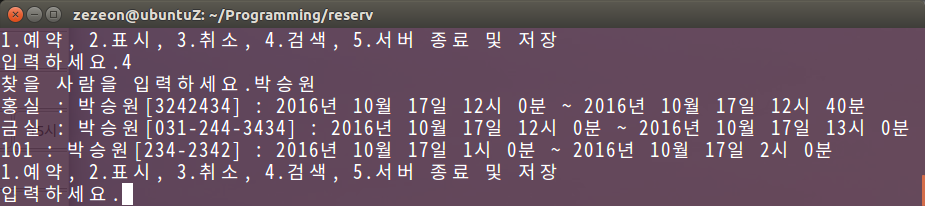
\includegraphics[width=0.9\textwidth]{con.png}

\section{클라이언트 프로그램}
클라이언트는 서버와 통신하며 명령행에서 모든 인자를 입력하여 사용한다.
프론트엔드를 위한 base 프로그램이지만, 독립적으로도 사용할 수 있다.

./client [option] [시간] [시설] 

의 형식으로 사용한다.

option에는 reserve, cancel, display, end가 올 수 있다.

client reserve 박승원 031-000-0000 2016 10 11 12 0 2016 10 11 14 30 청실  

로 실행하면 16년 10/11 12시부터 2시 30분까지 박승원[연락처:031-000-0000]으로 예약된다.

client cancel 박승원 2016 10 11 12 0 청실

은 위의 예약을 취소한다.

client display 청실 

은 청실의 모든 예약을 보여준다.

client end

는 서버를 종료하고 예약을 저장한다.
\end{document}
